\documentclass[10pt]{article}

\usepackage[margin=0.78in]{geometry}
\usepackage{amsmath,amssymb}
\usepackage{tikz}
\usetikzlibrary{arrows.meta,calc,positioning}
\usepackage{microtype}
\usepackage{hyperref}
\usepackage{float}
\hypersetup{
  colorlinks=true,
  urlcolor=blue!55!black,
  linkcolor=blue!55!black
}
\usepackage{multicol}
\setlength{\parindent}{0pt}
\setlength{\parskip}{3pt}
\setlength{\abovedisplayskip}{6pt plus 2pt minus 2pt}
\setlength{\belowdisplayskip}{6pt plus 2pt minus 2pt}
\setlength{\abovedisplayshortskip}{4pt plus 1pt minus 1pt}
\setlength{\belowdisplayshortskip}{4pt plus 1pt minus 1pt}

\title{\sc Camera Shell Design: drag estimates}
\author{\sc M. Nichitiu | MIT RT Simulations\vspace{3em}}
\date{}%\sc \today}

\begin{document}
\begin{multicols}{2}
	\maketitle
\vspace{-3.0em}
\begin{figure}[H]
\centering
\vspace{3.6em}

\includegraphics[width=0.35\textwidth]{logos/rtlogo.pdf}	
\end{figure}

\end{multicols}



\textit{Scope.} This is an inviscid, two-dimensional wedge estimate for a camera-shell
compression face. It is useful for selecting a slender transition angle, but it is not
a flight qualification analysis: skin friction, base drag, three-dimensional interference,
thermal loads, structural loads, and stability are omitted.

\section*{1. Governing result}

For a shell face of area $S$ inclined by angle $\theta$ to the rocket/fuselage axis,
with approximately uniform post-shock pressure $p_2$, the axial wave-drag component is

\begin{equation}
  \boxed{D_{\mathrm w} = (p_2-p_\infty)S\sin\theta}
  \label{eq:drag-result}
\end{equation}

where $p_\infty$ is the freestream static pressure. The pressure $p_2$ is obtained from
the attached oblique-shock solution:

\begin{align}
  \tan\theta &=
  2\cot\beta\,
  \frac{M_\infty^2\sin^2\beta-1}
  {M_\infty^2\left(\gamma+\cos 2\beta\right)+2},
  \label{eq:theta-beta-m}\\[3pt]
  \frac{p_2}{p_\infty} &=
  1+\frac{2\gamma}{\gamma+1}
  \left(M_\infty^2\sin^2\beta-1\right).
  \label{eq:pressure-ratio}
\end{align}

For the illustrative case $M_\infty=3$, $\gamma=1.4$, and $\theta=10^\circ$,
the weak attached-shock solution is
$\beta\simeq27.4^\circ$, $p_2/p_\infty\simeq2.05$, and
$C_p=(p_2-p_\infty)/q_\infty\simeq0.167$.

\section*{2. Shock and drag schematic}

The left panel shows the sharp-wedge idealization used by Eqs.~\eqref{eq:theta-beta-m}
and~\eqref{eq:pressure-ratio}. The right panel shows what changes when the shell nose is
rounded: the shock generally detaches, and its stand-off distance depends on nose radius
and three-dimensional geometry rather than on the wedge relation alone.

\begin{figure}[ht]
\centering
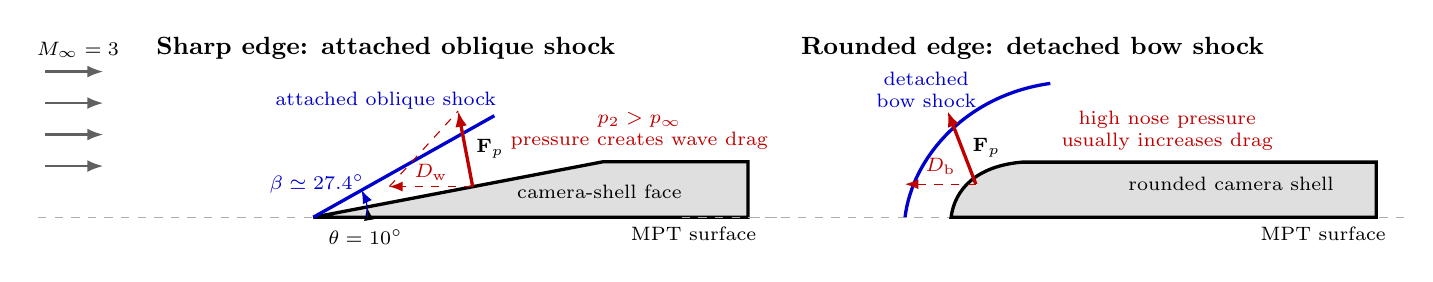
\begin{tikzpicture}[
    >=Latex,
    body/.style={draw=black, very thick, fill=gray!25},
    shock/.style={draw=blue!80!black, very thick},
    flow/.style={draw=gray!75!black, -{Latex[length=2mm]}, thick},
    pressure/.style={draw=red!75!black, -{Latex[length=2mm]}, very thick},
    construction/.style={draw=gray!65, dashed, thin},
    label/.style={font=\scriptsize},
]

% ---------------------------------------------------------
% Sharp leading edge / attached oblique shock
% ---------------------------------------------------------
\begin{scope}[xscale=0.92]
  \node[font=\small\bfseries] at (1.0,2.15)
    {Sharp edge: attached oblique shock};

  \draw[construction] (-3.8,0) -- (6.4,0);
  \node[label,below] at (5.25,0) {MPT surface};

  \draw[body]
    (0,0) -- (4,0.705) -- (6,0.705) -- (6,0) -- cycle;
  \node[label,align=center] at (3.95,0.32)
    {camera-shell face};

  \draw[shock] (2.5,1.29) -- (0,0);
  \node[label,blue!80!black] at (1,1.48)
    {attached oblique shock};

  \foreach \y in {0.65,1.05,1.45,1.85}
    {\draw[flow] (-3.7,\y) -- (-2.9,\y);}
  \node[label,above] at (-3.25,1.9) {$M_\infty=3$};

  \draw[black,->] (0.75,0) arc (0:10:0.75);
  \node[label] at (0.72,-0.25) {$\theta=10^\circ$};

  \draw[blue!80!black,->] (0.75,0) arc (0:27.4:0.75);
  \node[label,blue!80!black] at (0.05,0.42)
    {$\beta\simeq27.4^\circ$};

  \coordinate (P) at (2.2,0.39);
  \coordinate (F) at (2.0,1.35);
  \coordinate (Dx) at (1.05,0.39);
  \draw[pressure] (P) -- (F) node[midway,right,label] {$\mathbf F_p$};
  \draw[red!75!black,dashed,->] (P) -- (Dx)
    node[midway,above=-0.5mm,label] {$D_{\mathrm w}$};
  \draw[red!75!black,dashed] (Dx) -- (F);
  \node[label,red!75!black,align=center] at (4.5,1.10)
    {$p_2>p_\infty$\\pressure creates wave drag};
\end{scope}

% ---------------------------------------------------------
% Rounded leading edge / detached bow shock
% ---------------------------------------------------------
\begin{scope}[xshift=8.1cm,xscale=0.90]
  \node[font=\small\bfseries] at (1.15,2.15)
    {Rounded edge: detached bow shock};

  \draw[construction] (-3.8,0) -- (6.4,0);
  \node[label,below] at (5.25,0) {MPT surface};

  \draw[body]
    (0,0)
    .. controls (0.05,0.35) and (0.35,0.65) .. (1.0,0.70)
    -- (6,0.70) -- (6,0) -- cycle;
  \node[label,align=center] at (3.95,0.43)
    {rounded camera shell};

  \draw[shock]
    (-0.65,0)
    .. controls (-0.55,0.75) and (0.20,1.55) .. (1.40,1.70);
  \node[label,blue!80!black,align=center] at (-0.35,1.62)
    {detached\\bow shock};

  \coordinate (P2) at (0.35,0.42);
  \coordinate (F2) at (-0.05,1.35);
  \coordinate (Dx2) at (-0.65,0.42);
  \draw[pressure] (P2) -- (F2) node[midway,right,label] {$\mathbf F_p$};
  \draw[red!75!black,dashed,->] (P2) -- (Dx2)
    node[midway,above,label] {$D_{\mathrm b}$};
  \node[label,red!75!black,align=center] at (3.05,1.10)
    {high nose pressure\\usually increases drag};
\end{scope}

\end{tikzpicture}
\caption{Schematic of the shock system and pressure-drag mechanism. The shock locations
are illustrative and are not to scale.}
\label{fig:shock-drag}
\end{figure}

\small
\paragraph{Freestream pressure versus altitude.}
For a standard atmosphere, the entire 5,000--30,000 ft interval lies in the troposphere.
With $h_{\rm ft}$ denoting geometric altitude in feet, $h_{\rm m}=0.3048h_{\rm ft}$,
$T_0=288.15\,\mathrm{K}$, $p_0=101325\,\mathrm{Pa}$, lapse rate
$L=0.0065\,\mathrm{K/m}$, $R=287.05\,\mathrm{J/(kg\,K)}$, and
$g_0=9.80665\,\mathrm{m/s^2}$,
using the NASA standard-atmosphere model
\href{https://www1.grc.nasa.gov/beginners-guide-to-aeronautics/earth-atmosphere-equation-english/}
{given here}.

\begin{equation}
  p_\infty(h_{\rm ft})
  =101325\left(1-6.8756\times10^{-6}h_{\rm ft}\right)^{5.2559}\ \mathrm{Pa},
  \qquad 5000\le h_{\rm ft}\le30000.
  \label{eq:pressure-altitude}
\end{equation}

\begin{samepage}
At $M_\infty=3$ and $\gamma=1.4$, $q_\infty=\tfrac12\gamma M_\infty^2p_\infty
=6.3p_\infty$. Representative values are:

\begin{center}
\small\renewcommand{\arraystretch}{1.3}
\begin{tabular}{c|rrrrrr}
  altitude (ft) & 5,000 & 10,000 & 15,000 & 20,000 & 25,000 & 30,000 \\
  \hline
  $p_\infty$ (kPa) & 84.3 & 69.7 & 57.2 & 46.6 & 37.6 & 30.1 \\
  $q_\infty$ at $M=3$ (kPa) & 531.1 & 439.0 & 360.2 & 293.3 & 236.9 & 189.6
\end{tabular}
\end{center}
\end{samepage}

\paragraph{Example drag density at 5,000 ft.}
For $h=5000\,\mathrm{ft}$, $\theta=10^\circ$, and the weak-shock result
$p_2/p_\infty=2.0545$,

\begin{equation}
  \frac{D_{\mathrm w}}{S}
  =(p_2-p_\infty)\sin\theta
  =\left[(2.0545-1)(84.3\,\mathrm{kPa})\right]\sin10^\circ
  \simeq 15.4\,\mathrm{kPa}
  =15.4\,\mathrm{kN/m^2}
  \quad (\simeq 2.24\,\mathrm{psi}).
  \label{eq:drag-density-example}
\end{equation}

\paragraph{Last year's design.}
For the previous design, $S=9\times10^{-4}\,\mathrm{m^2}$ and $\theta=8^\circ$.
At 5,000 ft and $M_\infty=3$, the weak-shock solution gives
$\beta\simeq25.61^\circ$ and $p_2/p_\infty\simeq1.7953$. Thus the estimated full
axial wave drag on the shell face is

\begin{equation}
  D_{\mathrm w}
  =\left[(1.7953-1)(84.3\,\mathrm{kPa})\right]
    (9\times10^{-4}\,\mathrm{m^2})\sin8^\circ
  \simeq 8.40\,\mathrm{N}
  \quad (\simeq1.89\,\mathrm{lbf}).
  \label{eq:last-year-drag}
\end{equation}

For comparison, CFD results for last year's design gave
$D_{\mathrm{CFD}}\simeq 7\pm3\,\mathrm{N}$.

\begin{figure}[H]
\centering
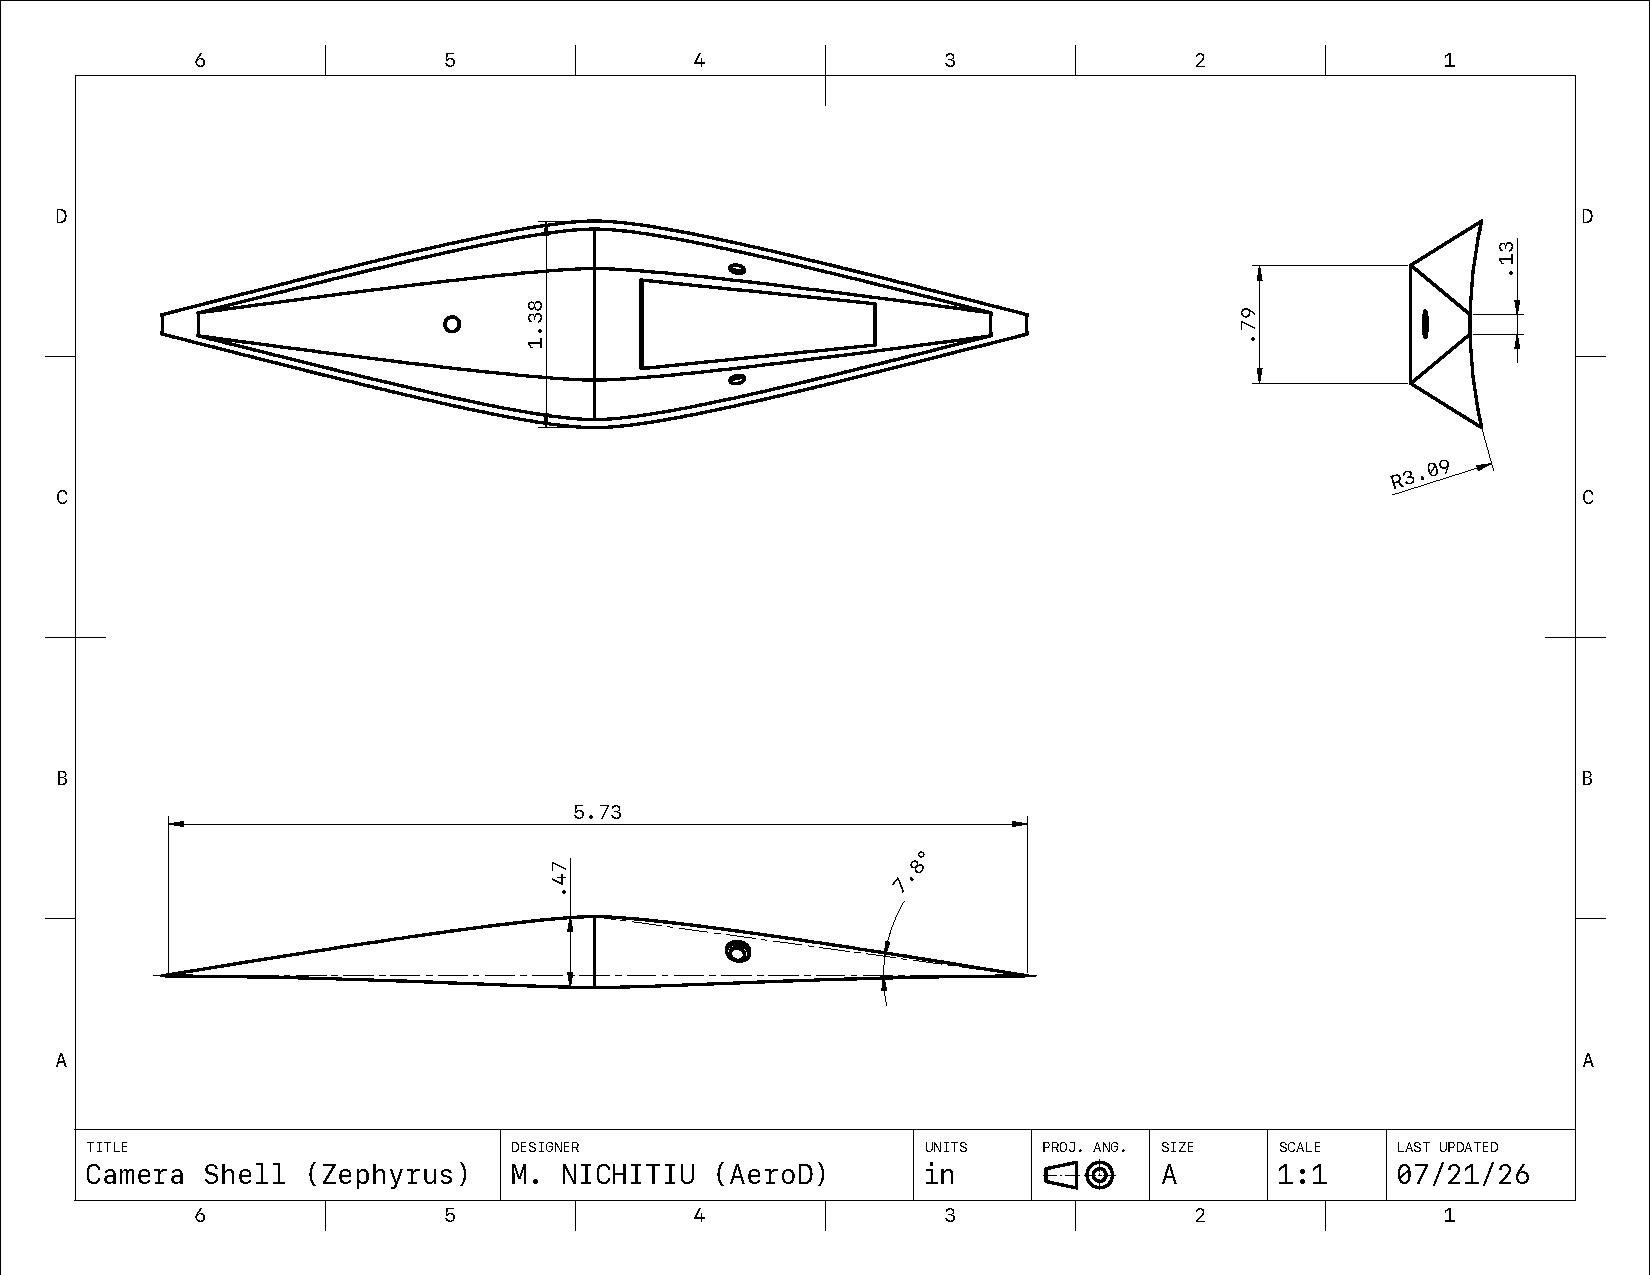
\includegraphics[width=\textwidth]{camerashellsketch.pdf}	
\caption{Engineering Sketch of the Camera Shell for \it Project Zephyrus.}
\end{figure}
\begin{figure}[H]
\centering
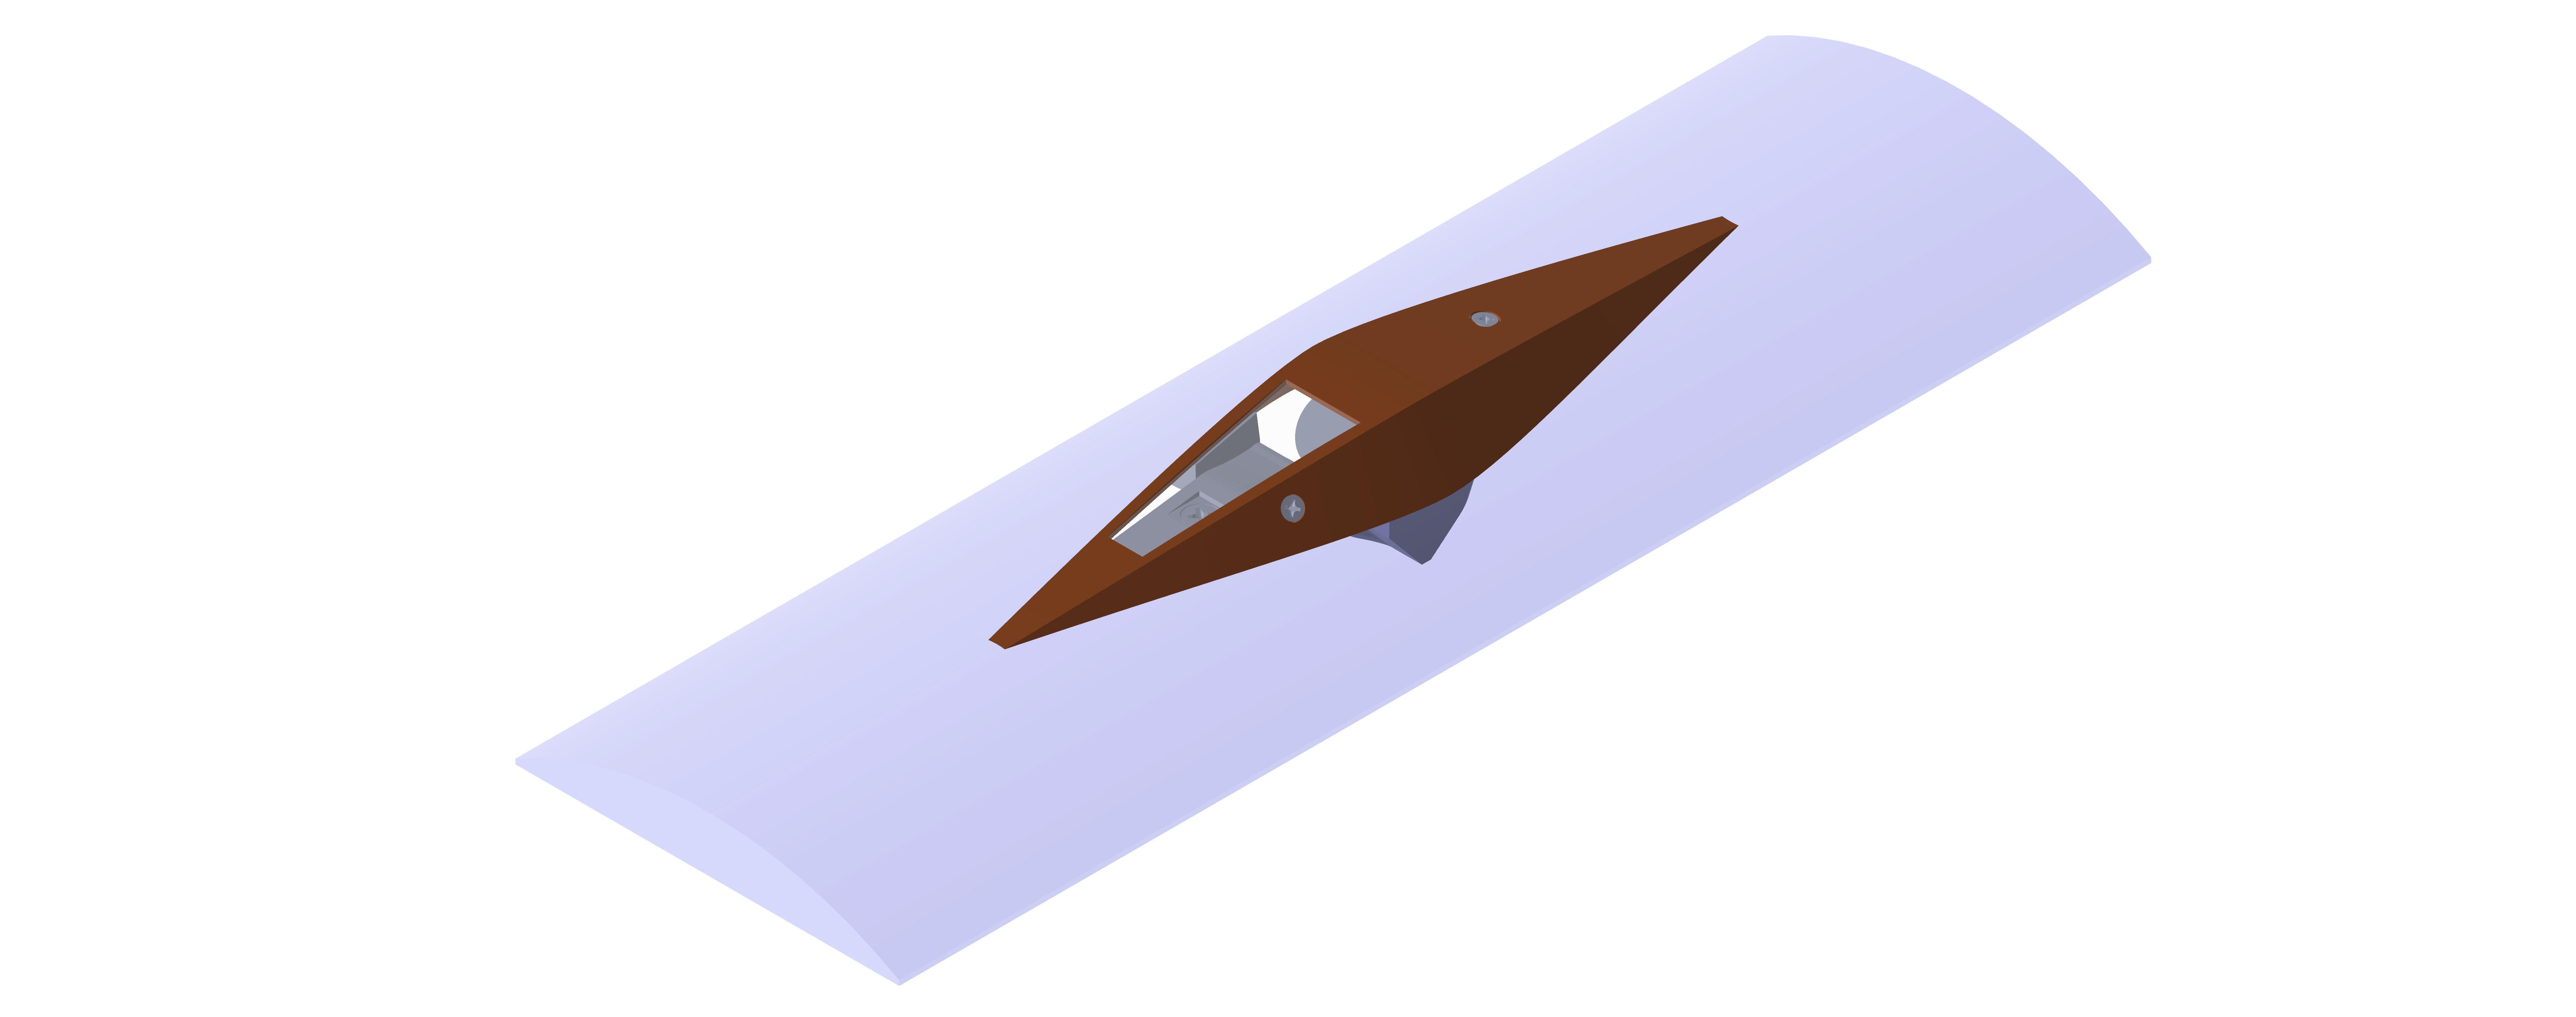
\includegraphics[width=1\textwidth]{render}	
\caption{Render of the Camera Shell for \it Project Zephyrus.}
\end{figure}


\setlength{\abovedisplayskip}{1pt plus 1pt minus 1pt}
\setlength{\belowdisplayskip}{1pt plus 1pt minus 1pt}
\setlength{\abovedisplayshortskip}{1pt plus 1pt minus 1pt}
\setlength{\belowdisplayshortskip}{1pt plus 1pt minus 1pt}

\footnotesize
\section*{3. Derivation of the drag relation}

Let $\hat{\boldsymbol{x}}$ point downstream, in the direction of the external flow in
the body-fixed frame, and let $\boldsymbol{n}$ be the outward unit normal of the shell.
The pressure traction on a surface element $dS$ is

\begin{equation}
  d\boldsymbol{F}=-p\,\boldsymbol{n}\,dS.
\end{equation}

The uniform freestream pressure produces no net force on a closed body, so it is useful
to work with the pressure difference $\Delta p=p-p_\infty$. The drag magnitude, defined
positive opposite the flow direction, is therefore

\begin{equation}
  D=-\boldsymbol{F}\cdot\hat{\boldsymbol{x}}
   =\int_S (p-p_\infty)n_x\,dS,
  \qquad n_x=\boldsymbol{n}\cdot\hat{\boldsymbol{x}}.
  \label{eq:integral-drag}
\end{equation}

For a sharp, uniform compression face inclined at $\theta$ to the axis, the face normal
has an axial projection $n_x=\sin\theta$. Oblique-shock theory treats the surface
pressure as uniform at $p_2$. Substituting both facts into Eq.~\eqref{eq:integral-drag}
gives

\begin{equation}
  D_{\mathrm w}=\int_S(p_2-p_\infty)\sin\theta\,dS
  =(p_2-p_\infty)S\sin\theta,
\end{equation}

which is Eq.~\eqref{eq:drag-result}.

Using the freestream dynamic pressure

\begin{equation}
  q_\infty=\frac{1}{2}\gamma p_\infty M_\infty^2,
\end{equation}

the corresponding pressure-drag coefficient is

\begin{equation}
  C_{D,\mathrm w}
  =\frac{D_{\mathrm w}}{q_\infty S_{\mathrm{ref}}}
  =C_p\frac{S}{S_{\mathrm{ref}}}\sin\theta,
  \qquad
  C_p=\frac{p_2-p_\infty}{q_\infty}.
  \label{eq:cd}
\end{equation}

The pressure $p_2$ follows by treating the component of Mach number normal to the shock
as a normal-shock problem:

\begin{equation}
  M_{n,\infty}=M_\infty\sin\beta,
  \qquad
  \frac{p_2}{p_\infty}=1+\frac{2\gamma}{\gamma+1}
  \left(M_{n,\infty}^2-1\right),
\end{equation}

while the flow-turning requirement gives the $\theta$-$\beta$-$M$ relation in
Eq.~\eqref{eq:theta-beta-m}. The weak-shock root is normally selected when it exists.

\enlargethispage{2\baselineskip}
\section*{4. Angle selection}

For small angles, the pressure rise across a weak oblique shock is approximately
proportional to $\theta$, while $\sin\theta\approx\theta$. Consequently,

\begin{equation}
  D_{\mathrm w}\propto\theta^2
  \qquad (\theta\ll1).
\end{equation}

Therefore oblique-shock theory alone gives no nonzero optimum angle: if the shell height
is fixed and its axial transition length can grow, drag is reduced by making the shell
more slender. For a prescribed height $h$ and transition length $L$,

\begin{equation}
  \theta=\arctan\!\left(\frac{h}{L}\right).
\end{equation}

{\scriptsize
Use the smallest practical angle with a smooth, tangent-continuous fairing. Rounded or
blunt shells require CFD or detached-bow-shock analysis; $\Delta x$ in Fig.~\ref{fig:shock-drag}
is illustrative rather than determined by the sharp-wedge equations.

\par\vspace{1pt}
\textit{Sources:}
NASA Glenn, \href{https://www.grc.nasa.gov/www/BGH/oblique.html}{oblique-shock relations};
NASA Glenn, \href{https://www.grc.nasa.gov/www/wind/valid/wedge/wedge.html}{Mach 2.5 wedge validation};
NASA Glenn, \href{https://www1.grc.nasa.gov/beginners-guide-to-aeronautics/earth-atmosphere-equation-english/}{standard-atmosphere model}.
\par}

\end{document}
